\documentclass{article}
\usepackage{graphicx}

\begin{document}

\title{IOUtil}
\author{Thomas Radke, Gabrielle Allen}
\date{June 2000}
\maketitle

\section{Introduction}

This document details the thorns provided in the standard Cactus 
distribution for the output of grid variables, and describes how to 
set parameters for I/O and checkpointing using these thorns.

Input and Output of data (I/O) in Cactus is provided by infrastructure thorns,
which interact with the flesh via a fixed interface, which is described in 
the Users Guide. 
The standard release of Cactus contains a number of thorns 
which provide parallel I/O using a variety of data formats and methods. 
All these provided I/O methods use thorn {\tt CactusBase/IOUtil} which 
provides general utilities for I/O (such as parsing parameter strings to
decide which variables to output), and a general set of parameters which
are inherited by the different I/O methods (such as the output directory). 
Thorn {\tt IOUtil} by itself provides no I/O methods.

More information about I/O and Visualisation of Cactus data can be found in 
the individual I/O thorns, and in the {\tt Visualization-HOWTO} available 
on the Cactus web pages.

\section{I/O methods in Cactus}

Cactus has several I/O modes for the output of grid variables in different 
formats.
Each I/O method comes with its own parameters by which it can be customised,
and all methods are registered with the flesh, satisfying the 
Cactus API, allowing them to be called directly from application thorns. 
An I/O method registers itself with the flesh along with it's name, and 
these registered names are the labels we now use to describe the various
methods. 


\begin{table}
\label{one}
\begin{tabular}{|l|p{4.5cm}|l|}
  \hline
  {\bf I/O method} & {\bf Description} & {\bf Providing Thorn}\\
  \hline
  {\tt Scalar} & 
  output of scalars or grid array reductions in xgraph or gnuplot format & 
  {\tt CactusBase/IOBasic}
\\
  {\tt Info}      & 
  screen output of scalars or grid array reductions & 
  {\tt CactusBase/IOBasic}
\\
&&\\
  {\tt IOASCII\_1D} & 
  1D line output of grid arrays in xgraph or gnuplot format & 
  {\tt CactusBase/IOASCII}
\\
  {\tt IOASCII\_2D} & 
  2D slice output of grid arrays in gnuplot format & 
  {\tt CactusBase/IOASCII}
\\
&&\\
  {\tt IOHDF5\_2D} & 
  2D slice output of grid arrays in HDF5 format & 
  {\tt CactusPUGHIO/IOHDF5}
\\
  {\tt IOHDF5\_3D} & 
  full 3D output of grid arrays in HDF5 format & 
  {\tt CactusPUGHIO/IOHDF5}
\\
&&\\
  {\tt IOFlexIO\_2D} & 
  2D slice output of grid arrays in FlexIO format & 
  {\tt CactusPUGHIO/IOFlexIO}
\\
  {\tt IOFlexIO\_3D} & 
  full 3D output of grid arrays in HDF5 format & 
  {\tt CactusPUGHIO/IOFlexIO}
\\
  \hline
\end{tabular}
\caption{Standard I/O methods provided with the Cactus distribution}
\end{table}

The standard provided Cactus I/O methods are shown in Table~\ref{one}.
As described above, each of these I/O thorns inherit parameters from thorn 
{\tt CactusBase/IOUtil}, which must be included in your ThornList
and activated in your parameter files before any of these I/O methods 
can be used. {\tt CactusBase/IOUtil} allows you to set the default 
behaviour for all the I/O methods described above, for examples, setting
the parameter {\tt IO::out\_every=1} will result in any chosen I/O method
providing output on each iteration. The default behaviour can be overriden
by specific parameters for each method.
For example, you may want scalar and 1D output at every iteration
but computationally expensive 3D output only every 10th iteration, 
with these files going into another directory on a scratch partition.

\section{External Packages}

NOTE: This section will not be filled out properly until the new treatment of external 
packages is implemented.

Some of the I/O methods used by Cactus require that external packages are installed and available 
on your machine. 

\begin{itemize}

\item{\tt HDF5} {\bf Hierachical Data Format}\\
{\tt http://hdf.ncsa.uiuc.edu/}

\item{\tt IEEEIO} \\
{\tt http://zeus.ncsa.uiuc.edu/}

\end{itemize}

\section{Standard Parameters}

Here we describe a few of the standard parameters used by {\tt IOUtil}
to control output. 
\begin{itemize}

\item{\tt IO::outdir}\\
  The name of the directory to be used for output. All the I/O 
  methods described here will write by default to this directory. 
  Individual methods have parameters
which can direct their output to a different directory.

\item{\tt IO::out\_every}\\
  How often, in terms of iterations, each of the Cactus I/O methods will
  write output. Again, individual methods can set there own parameter 
  to override this. The default is to never write output.
\end{itemize}

\section{Manipulating Parameter Files}

Thorn {\tt CactusBase/IOUtil} can also manage and manipulate parameter 
files, using the parameter {\tt IO::parfile\_write} to 

\begin{itemize}

  \item{\tt IO::parfile\_write="copy"} This is the default option,
  and makes an exact replica of the input parameter file in the
  standard output directory (this is particularly useful when the
  output directory is going to be archived).

  \item{\tt IO::parfile\_write="generate"} Generate a new parameter
  file from runtime information, containing the Cactus version, the
  name of the original parameter file, the run time/date, the host to
  run on, and the number of processors - all on comment
  lines. Following this the parameter file contains the ActiveThorns
  list plus a sorted list of all active thorns' parameters which have
  been set in the original parameter file.

  \item{\tt IO::parfile\_write="no"} Switch off writing of a new 
	parameter file.

\end{itemize}

The name of the new parameter file defaults to the original filename, 
unless the parameter {\tt IO::parfile\_name} is set. Note that if a file
already exists with the chosen name it will not be overwritten.
  

\section{I/O modes}
\label{iomodes}
For a run on multiple processors, scalar, 1D, and 2D output will always be 
written from only processor zero (that is, required data from all other
processors will be sent to processor zero, who then outputs all the gathered
data).
For 3D output this may become a quite expensive operation since output
by only a single processor will probably result in a I/O bottleneck and delay
further computation. 
For this reason Cactus offers different I/O modes for 3D output which can be
controlled by the {\tt IO::out\_3Dmode} parameter, in combination with
 {\tt IO::out\_unchunked} and {\tt IO::out3D\_np}. These parameters allow
I/O to be optimised for your particular machine architecture and needs: 

\begin{itemize}
  \item {\tt IO::out3D\_mode = "onefile"}\\
    As for the 1D and 2D I/O methods, writing to file is performed only 
    by processor zero.
    This processor gathers all the output data from the other processors
    and writes to a single file. The gathered grid array data from each
    processor can be either
    written in chunks ({\tt IO::out3D\_unchunked = "no"}) with each chunk
    containing the data from a single processor, or collected into a
    single global array before writing ({\tt IO::out3D\_unchunked = "yes"}).
    The default is to write the data in chunks.
  \item {\tt IO::out3D\_mode = "np"}\\
    3D output is written in parallel for groups of processors. Each group
    consists of {\tt IO::out3D\_procs} processors which have assigned one
    I/O processor which writes the gathers data from the group and writes it
    to file. The chunked output will go into {\tt IO::out3D\_procs} files. 
    The default number of processors in a group is eight.
  \item {\tt IO::out3D\_mode = "proc"}\\
    This is the default method for 3D output.
    Every processor writes its own chunk of data into a separate output file.
\end{itemize}

Probably the single processor {\tt proc} mode is the most efficient 3D output mode on 
machines with a fast I/O subsystem and many I/O nodes (eg. an Origin 2000) 
because it provides the highest
parallelity for outputting data. Note that on very large numbers of processors
you mave have to fall back to {\tt np}, output from groups of processors, 
mode if the system limit of
maximum open file descriptors is exceeded (this is true for large jobs on a
 T3E).\\
While the {\tt np} and {\tt proc} I/O modes are fast for outputting large
amounts of data from all or a group of processors in parallel, they have
the disadvantage of writing chunked files. These files have to be 
{\tt recombined}
during a postprocessing phase so that the final unchunked data can be
visualized by standard tools. For that purpose a recombiner utility program is
provided by thorn {\tt CactusPUGHIO/IOFlexIO}.
Note that {\tt CactusPUGHIO/IOHDF5} does not provide such a utility yet. 

\section{Output of Hyperslab Data}

While some I/O methods ({\tt IOHDF5\_3D, IOFlexIO\_3D}) can dump the full
contents of a multidimensional CCTK variable, others such as
{\tt IOASCII\_1D} and {\tt IOASCII\_2D} will output only a subset of the data
(eg. 1D lines or 2D planes of 3D grid funtions).
Such a subset (called a {\it hyperslab}) is generally defined as an orthogonal
region into the multidimensional dataset, with a startpoint and a length in any
direction, and an optional downsampling factor.

Thorn {\tt IOUtil} defines a set of hyperslab parameters for all
I/O methods which determine the default positions of 1D line or 2D slice output
along the axes. I/O thorns can also define their own hyperslab parameters
which then will overwrite the defaults provided by {\tt IOUtil}.

\begin{itemize}
  \item {\tt IO::out\_[xyz]line\_[xyz]}\\
    specifies the slice center for 1D x,y,z-line output by coordinate values
    of the underlying physical grid
  \item {\tt IO::out\_[xyz]line\_[xyz]i}\\
    specifies the slice center of 1D x,y,z-line output by index points
    of the underlying computational grid
  \item {\tt IO::out\_[\{xy\}\{xz\}\{yz\}]plane\_[xyz]}\\
    specifies the slice center of 2D xy,xz,yz-plane output by coordinate values
    of the underlying physical grid
  \item {\tt IO::out\_[\{xy\}\{xz\}\{yz\}]plane\_[xyz]}i\\
    specifies the slice center of 2D xy,xz,yz-plane output by index points
    of the underlying computational grid
  \item {\tt IO::out3D\_downsample\_[xyz]}\\
    specifies the downsampling factor for 3D output in every direction
\end{itemize}

Setting the index points for the slice centers in a parameter file
has precedence over setting their location by coordinate values.
If nothing was specified the default values of {\tt IO::out\_[xyz]line\_[xyz]}
and {\tt IO::out\_[\{xy\}\{xz\}\{yz\}]plane\_[xyz]} will be used.
These are set to be all zeros which causes the output to go through the
coordinate system's origin or the closest grid point to this (see figure
\ref{default_1D_output} for an example).

\begin{figure}[ht]
\begin{center}
\includegraphics[width=6cm]{1Dlines_in_box.eps}
\includegraphics[width=6cm]{1Dlines_in_xyBitant.eps}
\end{center}
\caption{Default 1D {\it x,y,z}-line output for a 3D grid in box mode (left) and {\it xy}-bitant mode (right)}
\label{default_1D_output}
\end{figure}

Although they are not hyperslabs by the above definition, output of 1D
diagonals for 3D grid arrays is also supported by I/O method {\tt IOASCII\_1D}
but has the restriction that the line will always start in the bottom-left
corner of the computational grid and steadily rise by one grid point in
every direction (see figure \ref{default_diagonal_output} for an example).

\begin{figure}[ht]
\begin{center}
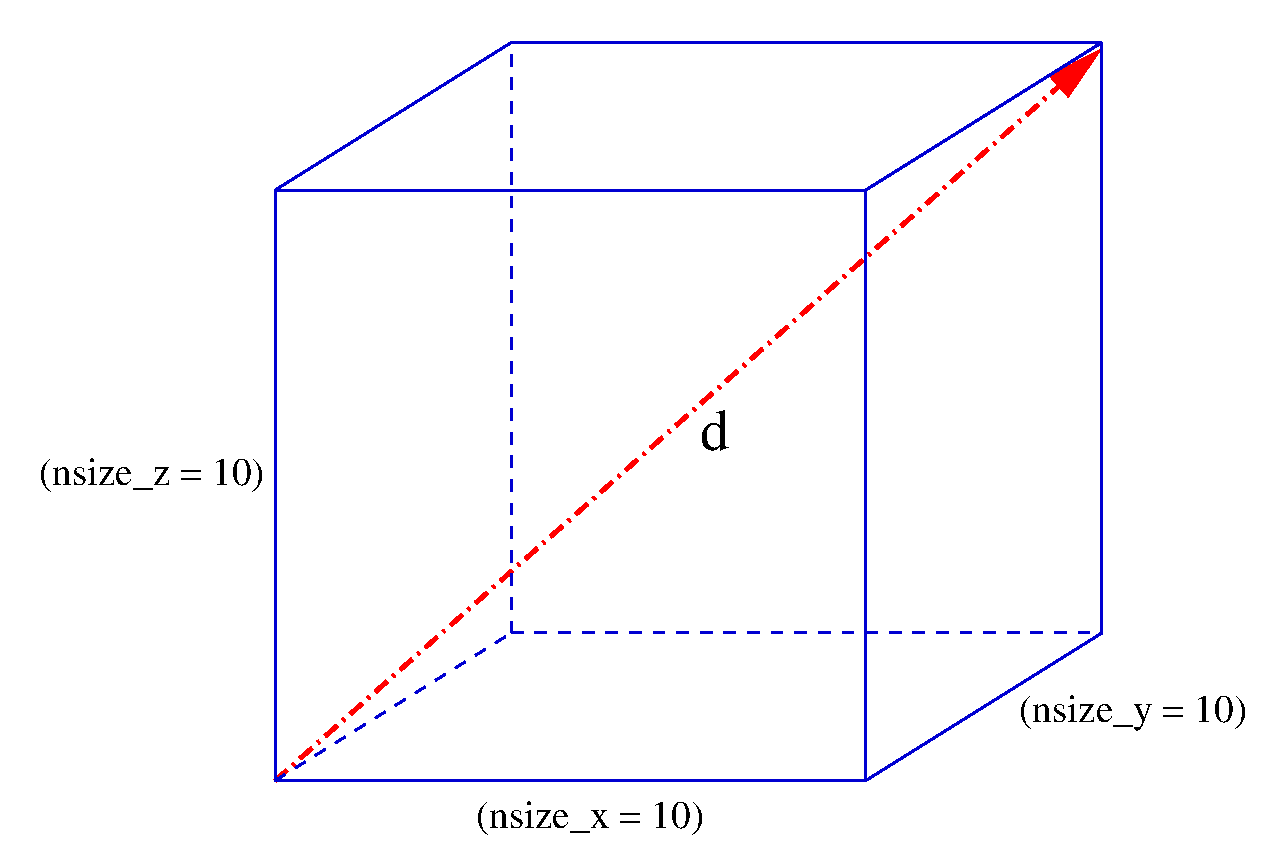
\includegraphics[width=6cm]{diagonal_in_cubic.eps}
\includegraphics[width=6cm]{diagonal_in_noncubic.eps}
\end{center}
\caption{1D diagonal output for a 3D cubical (left) and non-cubical (right)
computational grid}
\label{default_diagonal_output}
\end{figure}


\section{Checkpointing and Recovery in Cactus}

The I/O methods for 3D output also provide functionality for {\it checkpointing}
and {\it recovery}. A checkpoint is a snapshot of the current state of the 
simulation ({\it ie} the contents of all the grid variables and the parameter 
settings) at a chosen timestep. Each checkpoint is saved into a 
{\it checkpoint file} which can be used to restart a new simulation at a later
time, recreating the exact state at which it was checkpointed.\\
Checkpointing is especially useful when running Cactus in batch queue systems 
where jobs get only limited CPU time. A more advanced use of checkpointing 
would be to restart your simulation after a crash or a problem had developed,
using a  different parameter set recovering from the latest stable timestep. 
Additionally, for performing parameter studies,  compute-intensive
initial data can be calculated just once and saved in a checkpoint file 
from which each job can be started. \\

Again, thorn {\tt CactusBase/IOUtil} provides general checkpoint \& recovery
parameters. The most important ones are:
\begin{itemize}
  \item {\tt IO::checkpoint\_every}\\
    specifies how often to checkpoint in terms of iteration number
  \item {\tt IO::checkpoint\_file}\\
    holds the checkpoint filename
  \item {\tt IO::checkpoint\_dir}\\
    names the directory where checkpoint files are stored
  \item {\tt IO::checkpoint\_ID}\\
    boolean flag for checkpointing only initial data
  \item {\tt IO::recover}\\
    keyword parameter telling if/how to recover.\\
    Choices are {\tt "no"}, {\tt "manual"}, {\tt "auto"}, and {\tt "autoprobe"}.
  \item {\tt IO::recover\_file}\\
    filename of the recovery file
  \item {\tt IO::recovery\_dir}\\
    directory where the recovery file is located
\end{itemize}

To checkpoint your simulation, you need to enable checkpointing by setting
the Boolean parameter {\tt checkpoint}, for one of the 3D I/O methods to
{\tt yes}.
Checkpoint filenames consist of a basename (as specified in
{\tt IO::checkpoint\_file}) followed by {\tt ".chkpt.it\_$<$iteration\_number$>$"}
plus the file extension indicating the file format ({\tt ".ieee"} for IEEEIO
data from {\tt CactusPUGHIO/IOFlexIO}, or {\tt ".h5} for HDF5 data from
{\tt CactusPUGHIO/IOHDF5}).\\
Use the {\tt "manual"} mode to recover from a specific checkpoint file
by adding the iteration number to the basename parameter.

The {\tt "auto"} recovery mode will automatically
recover from the latest checkpoint file found in the recovery directory.
In this case {\tt IO::recover\_file} should contain the basename only.

The {\tt "autoprobe"} recovery mode is similar to the {\tt "auto"} mode
except that it would not stop the code if no checkpoint file was
found but only print a warning message and then continue with the
simulation. This mode allows you to enable checkpointing and recovery
in the same parameter file and use that without any changes to restart your
simulation. On the other hand, you are responsible now for making the
checkpoint/recovery directory/file parameters match -- a mismatch will not
be detected by Cactus in order to terminate it. Instead the simulation would
always start from initial data without any recovery.\\

Because the same I/O methods implement both output of 3D data and
checkpoint files, the same I/O modes are used (see Section~\ref{iomodes}). 
Note that the recovery routines in Cactus can process both chunked and 
unchunked checkpoint files if you restart on the same number of processors.
That's why you should always use one of the parallel I/O modes for 
checkpointing. If you want to restart on a different number of processors, you first need to 
{\it recombine} the data in the checkpoint file(s) to create a single file with
unchunked data.
Note that you can restart from your checkpoint file on a different machine.

\vskip .5cm
\noindent{\bf WARNING:}

\noindent
Checkpointing and recovery should {\bf always} be tested for a new thorn set. This is because
only Cactus grid variables and parameters are saved in a checkpoint file. If a thorn has made 
use of saved local
variables, the state of a recovered simulation may differ from the original run. To test 
checkpointing and recovery, simply perform one run of say 10 timesteps, and compare output data
with a checkpointed and recovered run at say the 5th timestep. The output data should match 
exactly if recovery was successful.

%%%%%%%%%%%%%%%%%%%%%%%%%%%%%%%%%%%%%%%%%%%%%%%%%%%%%%%%%%%%%%%%%%%%%%%%%%%%%%%
\section{Reading Data from Files into Cactus}

The very same routines which implement checkpointing/recovery functionality
in the {\tt IOHDF5} and {\tt IOFlexIO} thorns are also used to provide
filereader capabilities within Cactus. They enable a user to read variables,
which contents was written to files in HDF5 or IEEEIO data format, back into
Cactus at a later time. This is especially useful if compute-intensive
initial data is calculated only once and stored in a file. Such data
can then be read back in at startup and immediately used by following evolution
runs.

The following {\tt IOUtil} parameters exist to specify what variables should be
read from file(s) as initial data:

\begin{itemize}
  \item {\tt IO::recover\_ID\_files}\\
  list of files to read in as initial data (multiple filenames must be separated by spaces)\\
  The same file naming conventions (what I/O mode used, which iteration number)
  apply as for checkpoint files.
  \item {\tt IO::recover\_ID\_vars}\\
  list of CCTK variables to read in from the given initial data files (variables
  are identified by their full name, multiple variable names must be separated by spaces)\\
  This is useful if a datafile contains multiple variables but only some of
  them should be read. Thus it is possible to recover distinguished
  variables from a full checkpoint file. Note that if the file contains several
  timesteps of the same variable only the last one is taken.
\end{itemize}

Thorn {\tt IOUtil} also provides a filereader routine which can be called
by any application thorn at any time. It gets passed the equivalent information
to the filereader parameters, plus a pointer to the underlying CCTK grid hierarchy.

\begin{verbatim}
void IOUtil_RecoverVarsFromDatafiles (cGH *GH,
                                      const char *in_files,
                                      const char *in_vars);
\end{verbatim}

If data is to be imported from files which were not created by
{\tt IOHDF5} or {\tt IOFlexIO} it needs to be converted first into the
appropriate HDF5 or IEEEIO file format and the file layout
which either one of these thorns uses. This is described in detail in the
thorns' documentation, along with a simple C source file which can be used as a
template to build your own data converter program.


%%%%%%%%%%%%%%%%%%%%%%%%%%%%%%%%%%%%%%%%%%%%%%%%%%%%%%%%%%%%%%%%%%%%%%%%%%%%%%%
\section{Data Filenames and Filename Extensions}

The standard I/O thorns in Cactus make use of a consistent set of filenames
and extensions, which identify the variables and data format used in the file.
The filenames are listed in the following tables.
%The filenames are listed in Table~\ref{filename_table},
%and the extensions in Table~\ref{filename_extensions_table}

\begin{center}
\begin{table}[htb]
\label{filename_table}
\begin{tabular}{|l|l|}
  \hline
  {\bf I/O method}   & {\bf Filename for output of variable {\tt phi}}\\
  \hline
  {\tt Scalar}       & phi\_nm1.tl, phi\_nm2.tl phi\_max.tl phi\_min.tl\\
  {\tt Info}         & Provides no output file (the same data is available with {\tt Scalar} output)\\
  {\tt IOASCII\_1D}  & phi.xl, phi.yl, phi.zl, phi.dl\\
  {\tt IOASCII\_2D}  & phi\_2d\_xy.gnuplot, phi\_2d\_xz.gnuplot, phi\_2d\_yz.gnuplot\\
  {\tt IOHDF5\_3D}   & phi\_3d.h5\\
  {\tt IOFlexIO\_2D} & phi\_2d.ieee\\
  {\tt IOFlexIO\_3D} & phi\_3d.ieee\\
  \hline
\end{tabular}
\caption{Filenames used by standard I/O thorns}
\end{table}
\end{center}

\begin{center}
\begin{table}[htb]
\label{filename_extensions_table}
\begin{tabular}{|c|p{4.5cm}|l|}
\hline
{\bf Extension} & {\bf Description} & {\bf Thorn} \\
  \hline
 {\tt .xl} & 1D line plots in {\it x}-direction & {\tt CactusBase/IOASCII}\\
 {\tt .yl} & 1D line plots in {\it y}-direction & {\tt CactusBase/IOASCII}\\
 {\tt .zl} & 1D line plots in {\it z}-direction & {\tt CactusBase/IOASCII}\\
 {\tt .dl} & 1D diagonal line plots             & {\tt CactusBase/IOASCII}\\
 {\tt .tl} & traceline plots over time          & {\tt CactusBase/IOBasic}\\
  \hline 
\end{tabular}
\caption{File extensions used by the standard I/O thorns in the Cactus distribution}
\end{table}
\end{center}
 
\section{Example Parameter Files}

Here we give examples of the parameters for the different I/O methods.

\begin{itemize}
\item{\bf Screen Information {\tt info}}
\begin{verbatim}
ActiveThorns = "iobasic ioutil ..."

# Output using all methods on iteration 0, 10, 20, ...
io::out_every = 10            

# Group of variables to output to screen
iobasic::outinfo_vars = "evolve::vars"
\end{verbatim}

\item{\bf Scalar Output {\tt scalar}}
\begin{verbatim}
ActiveThorns = "iobasic ioutil ..."

# Output vars using scalar method on iteration 0, 10, 20, ...
iobasic::outscalar_every = 10            

# Group of variables to output to file
iobasic::outscalar_vars = "evolve::vars"
\end{verbatim}

\item{\bf ASCII 1D and 2D Output {\tt ioascii\_1d}, {\tt ioascii\_2d}}
\begin{verbatim}
ActiveThorns = "ioascii ioutil pughslab ..."

# Output vars using ascii 1d method on iteration 0, 10, 20, ...
ioascii::out1d_every = 10            

# Output vars using ascii 2d method on iteration 0, 50, 100, ...
ioascii::out1d_every = 100

# Group of variables to output to file for each method
iobasic::outscalar_vars = "evolve::vars"
\end{verbatim}

\item{\bf HDF5 3D Output {\tt iohdf5\_3d}}
\begin{verbatim}
ActiveThorns = "iohdf5 ioutil pughslab ..."

# Output vars using ascii 2d method on iteration 0, 100, 200, ...
iohdf5::out2d_every = 100            

# Output vars using ascii 3d method on iteration 0, 5, 10, ...
iohdf5::out3d_every = 5

# Standard I/O directory for 2D output
io::outdir = "test"

# Special I/O directory for 3D output
iohdf5::outdir3D = "/scratch/tmp"

# 3D Output unchunked to one file 
# (Only using a small number of processors)
io::out3D_mode = "onefile"
io::out3D_unchunked = "yes"

# Downsample 3D data by a factor of 3 in each direction
io::out3D_downsample_x = 3
io::out3D_downsample_y = 3
io::out3D_downsample_z = 3

# Group of variables to output to file for each method
iohdf5::out2D_vars = "evolve::vars"
iohdf5::out3D_vars = "evolve::vars"
\end{verbatim}


\item{\bf IEEEIO 2D and 3D Output {\tt ioflexio\_2d}, {\tt ioflexio\_3d}}
\begin{verbatim}
ActiveThorns = "ioflexio ieeeio ioutil pughslab ..."

# Output vars using 2D FlexIO method on iteration 0, 100, 200, ...
ioflexio::out2d_every = 100            

# Output vars using 3D FlexIO method on iteration 0, 5, 10, ...
ioflexio::out3d_every = 5

# Standard I/O directory for 2D output
io::outdir = "test"

# Special I/O directory for 3D output
ioflexio::outdir3D = "/scratch/tmp"

# 3D Output chunked to one file for every eight processors
# (Run on large number of processors)
io::out3D_mode = "np"
io::out3D_nproc = 8
io::out3D_unchunked = "no"

# Downsample 3D data by a factor of 3 in each direction
io::out3D_downsample_x = 3
io::out3D_downsample_y = 3
io::out3D_downsample_z = 3

# Group of variables to output to file for each method
ioflexio::out2D_vars = "evolve::vars"
ioflexio::out3D_vars = "evolve::vars"
\end{verbatim}

\item{\bf Checkpointing using IEEEIO}
\begin{verbatim}
ActiveThorns = "ioflexio ieeeio ioutil pughslab ..."

# Use IEEEIO data format 
ioflexio::checkpoint = "yes"

# Make a new checkpoint file every 300 iterations
io::checkpoint_every = 300

# Name and directory of checkpoint file
io::checkpoint_file = "run5"
io::checkpoint_dir  = "/scratch/tmp"
\end{verbatim}

\item{\bf Recovering from a checkpoint file}
\begin{verbatim}
ActiveThorns = "ioflexio ieeeio ioutil pughslab ..."

io::recover = "auto"

# Name and directory of checkpoint file
io::recover_file = "run5"
io::recover_dir  = "/scratch/tmp"
\end{verbatim}

\end{itemize}
\end{document}
